% Generated by plsimcount.pfseeds -- do not edit; regenerate instead.
% figure: B-order4-by-formula -- Every order-4 formula at measured r; median over seeds [1, 2, 3, 4, 5], bars = min..max
% metric=t gatebase=ct merged
% seed 1: git_commit=04cd66abb614bdc66fb48e891cef085a299e0ab1 git_dirty=False
% seed 2: git_commit=04cd66abb614bdc66fb48e891cef085a299e0ab1 git_dirty=False
% seed 3: git_commit=04cd66abb614bdc66fb48e891cef085a299e0ab1 git_dirty=False
% seed 4: git_commit=04cd66abb614bdc66fb48e891cef085a299e0ab1 git_dirty=False
% seed 5: git_commit=04cd66abb614bdc66fb48e891cef085a299e0ab1 git_dirty=False
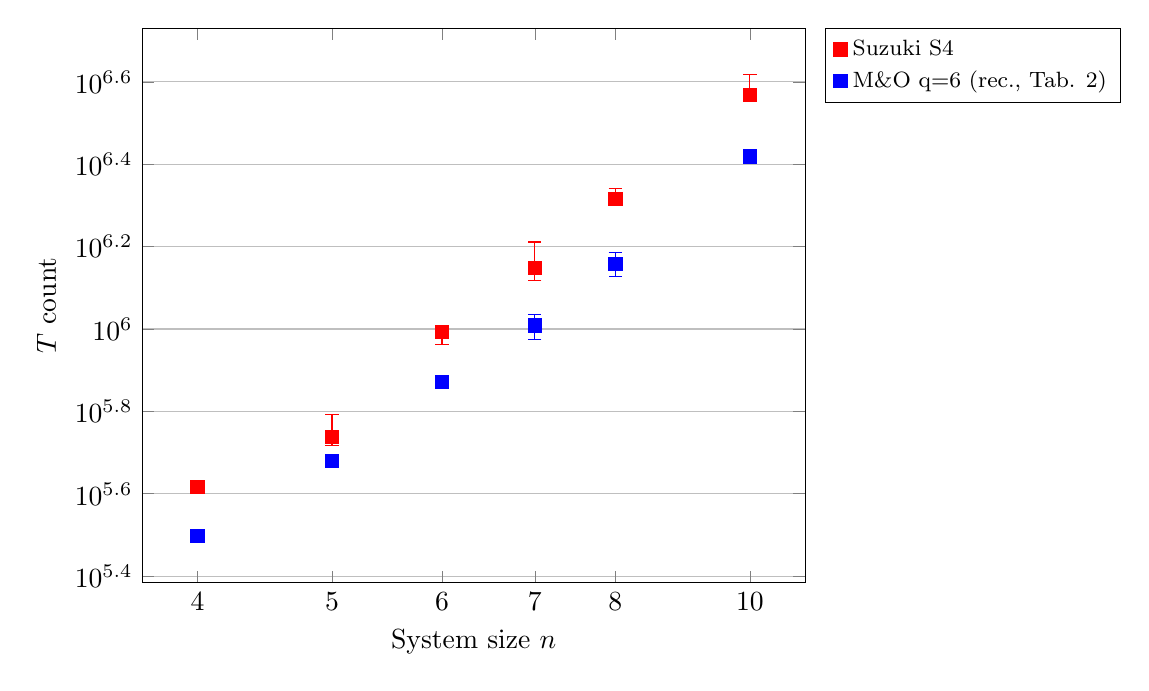
\begin{tikzpicture}
  \begin{loglogaxis}[
    width=10cm,
    xlabel={System size $n$},
    ylabel={$T$ count},
    xtick={4,5,6,7,8,10},
    xticklabels={4,5,6,7,8,10},
    ymajorgrids=true,
    legend pos=outer north east,
    legend cell align=left,
    legend style={font=\footnotesize},
  ]
    \addplot[only marks, red, mark=square*, mark size=2.4pt, mark options={solid, fill=red}, error bars/.cd, y dir=both, y explicit, error bar style={red}] coordinates {
      (4,413718) += (0,5272) -= (0,742)
      (5,547344) += (0,73710) -= (0,24870)
      (6,983882) += (0,33568) -= (0,66258)
      (7,1405320) += (0,220920) -= (0,90456)
      (8,2071296) += (0,126240) -= (0,50016)
      (10,3700064) += (0,450366) -= (0,118640)
    };
    \addlegendentry{Suzuki S4}
    \addplot[only marks, blue, mark=square*, mark size=2.4pt, mark options={solid, fill=blue}, error bars/.cd, y dir=both, y explicit, error bar style={blue}] coordinates {
      (4,314160) += (0,140) -= (0,840)
      (5,478632) += (0,1512) -= (0,10248)
      (6,744332) += (0,23116) -= (0,23804)
      (7,1018944) += (0,66240) -= (0,75708)
      (8,1435896) += (0,99144) -= (0,93708)
      (10,2628360) += (0,81736) -= (0,101208)
    };
    \addlegendentry{M\&O q=6 (rec., Tab. 2)}
  \end{loglogaxis}
\end{tikzpicture}
